\chapter{Snow Wetness Estimation From Full Polarimetric SAR Data}
\section{Introduction}

%
%High topographic mountain regions have great physical diversity with the environment. Particularly, the snow cover and its seasonal changes play an important role. The snow wetness in the Himalayan snowpack is an important parameter for snow-melt runoff modeling, snow avalanche risk assessment, climatology, hydro-power industry and weather forecasting. Shi $\emph{et al.}$ developed an inversion model to estimate snow wetness using SAR data based on the first-order scattering model considering both surface and volume scattering~\cite{Shi93}. The NASA/JPL airborne AIRSAR imaging polarimetric data was used in this study. However, the first-order scattering model do not apply for most natural surfaces as they are very rough on the radar wavelength scale. The Integral Equation Model (IEM) which is valid over a wider range of surface roughness is used for the inversion model to estimate snow wetness~\cite{Shi95}. The polarimetric space-borne Shuttle Imaging Radar Mission C-band (SIR-C) data was used for this study. The above method was modified to estimate snow wetness from conventional dual-polarization ENVISAT-ASAR data~\cite{Singh2010}. Statistical inversion model was also developed to retrieve snow wetness using ENVISAT-ASAR alternating polarization data~\cite{niang2007new}.

The availability of fully polarimetric Radarsat-2 data along with the advanced PolSAR decomposition techniques gives full freedom to utilize the complete polarimetric information for the development of new techniques for the estimation of geophysical parameters. In this chapter a new novel inversion model is proposed for snow wetness estimation from full-polarimetric SAR data based on Generalized Four Component Scattering Power Decomposition with unitary Transformations(G4U) technique.   
In wet snow, the surface and the volume are the dominant scattering mechanisms, therefore the generalized surface and the volume parameters are adopted. These parameters are then directly used to estimate the surface and the volume snow wetness. The effective snow wetness map is derived from the weighted average of both the wetness maps. The weights are derived from the normalized surface and volume scattering powers. The results obtained from the proposed method are validated with the near real time in-situ measurements with the satellite pass.

\section{Study Area and Data Used}

The study area comprised of snow cover over a bare flat terrain with sparse vegetation. This area is a part of the Beas and the Chandra Bhaga catchment which lies in the Kullu district of Himachal Pradesh, India. It is geographically located between the latitudes of 32$^\circ$ 15' N and 32$^\circ$ 30' N, and between the longitudes of 77$^\circ$ E and 77$^\circ$ 15' E. The Snow and Avalanche Study Establishment (SASE) under Ministry of Defense, Government of India, maintains three manual observatories at Solang, Dhundhi and Bhang which are located at an altitude of 2006 m, 2446 m and 2896 m respectively. According to the Forest Survey of India (FSI) report in 2011~\citep{FSI2011}, less than 17$\%$ areas in the state of Himachal Pradesh are covered with a dense vegetation. 

Field campaigns were conducted to collect near-real time in-situ measurements with the Radarsat-2 fine resolution quad polarimetric (FQ) data acquisitions for consecutive three winter seasons from 2012 to 2014 is shown in Table~\ref{table:data acquisition}. The study area is outlined in blue and the three observatories where the field campaigns were conducted are marked (green star) in Fig.~\ref{fig:study_area}. The 3x3 coherency matrix was generated from the single-look complex Radarsat-2 full-polarimetric SAR data. A multi looking factor of 3 in the range direction and 4 in the azimuth direction were used to make the square pixel and the Lee-Refined filter is applied to remove the speckle noise. The local incidence angle map is generated while performing the Range–Doppler terrain correction using the ASTER GDEM and the Layover/Shadow areas were also masked before applying the methodologies. 

The snow fork instrument was used in the field to measure the snow wetness in this study as shown in figures~\ref{fig:snow_cover_area}(a), (b), (c), (d). The snow fork is a portable instrument which measures the resonant frequency, attenuation and the 3-db bandwidth~\cite{sihvola1986snow}. These measurements are then used to calculate the complex dielectric constant of snow. The snow density and the wetness are calculated using semi-empirical equations. The measurements from this instrument are reliable as it does not compress the snowpack and the measurements are easily repeatable and the results can be checked by calibration measurement in the air. 

Each snow pits were dug around 30-40 cm in depth. The fork was completely inserted in every 5 cm depth interval of the snowpack and the snow wetness measurements were recorded. As per literatures, microwave C-band signal normally penetrate through the snowpack to a maximum by 15 to 20 cm in low to moderate snow wetness conditions. So, for validation purpose, the average snow wetness measurement for the top 20 cm snow depth were considered as a ground truth at each point.
\begin{figure*}[!h]
	\centering
	\includegraphics[width=\columnwidth]{Figures/sa_final}
	\caption{Study area with location of the three observatories.}
	\label{fig:study_area}
\end{figure*}

\begin{figure*}[!h]
	\centering
	\subfloat[]{\includegraphics[width=0.48\textwidth]{Figures/aa1_opt}} \hspace{1mm}
	\subfloat[]{\includegraphics[width=0.48\textwidth]{Figures/aa2_opt}} \\
	\subfloat[]{\includegraphics[width=0.48\textwidth]{Figures/aa3_opt}} \hspace{1mm}
	\subfloat[]{\includegraphics[width=0.48\textwidth]{Figures/aa4_opt}} \\
	\caption{Snow cover area along with field measurements.}
	\label{fig:snow_cover_area}
\end{figure*}

\begin{table}[!h]
	\caption{Data Acquisition Table}
	\begin{center}
		\begin{tabular}{| c | c | p{3cm} | c | p{2cm} |} \hline
			No. & Date & Acquisition Time (UTC+5:30h) & Pass & Incidence Angle ($^\circ$) \\ \hline \hline
			1 & 07 Feb 2012 & 6:18 AM & Descending & 41.9-43.3\\ \hline
			2 & 14 Feb 2012 & 6:14 AM & Descending & 46.8-48.0\\ \hline
			3 & 06 Feb 2013 & 6:25 PM & Ascending & 39.2-40.7\\ \hline
			4 & 08 Feb 2013 & 6:14 AM & Descending & 46.0-47.2\\ \hline
			5 & 18 Feb 2014 & 6:29 PM & Ascending & 44.4-45.7\\ \hline
			6 & 20 Feb 2014 & 6:18 AM & Descending & 41.0-42.4\\ \hline
		\end{tabular}
	\end{center}
	\label{table:data acquisition}
\end{table}

\section{Methodology}

%%Polarimetric target decomposition is a technique to characterize scattering mechanisms from polarimetric synthetic aperture radar (SAR) data. Target decomposition techniques can be broadly classified into two categories: (1) coherent decomposition techniques which utilize the information contained in a target scattering matrix [S], and (2) incoherent decomposition techniques which utilize the second-order statistics in terms of covariance matrices ([C] or [T]) derived from the scattering matrix [S]. Furthermore, incoherent decomposition techniques can be subdivided into eigenvalue/eigenvector based, and model-based. Eigenvalue/eigenvector based decompositions provide a unique solution in terms of the scattering mechanisms~\cite{CLOUDE97,TOUZI2007}, while the solutions provided by the model based decompositions depend on the assumptions made about the physical scattering model. Model-based decompositions have gained considerable attention after the initial work of Freeman-Durden~\cite{freeman98}. This decomposition assumes the target to be reflection symmetric. This assumption states that the co-polarized and the cross-polarized components are always uncorrelated. This assumption was later relaxed in the Yamaguchi decomposition~\cite{Yamaguchi2005}. which included the helical scattering as a fourth component. These two decompositions are widely used in literature because of their simplicity and computational ease.
%%
%%A major advancement was made with the orientation compensation application in model-based decompositions. This was necessary because of the fact that a target with different orientations in the plane orthogonal to the radar line of sight (LOS) will have different polarimetric responses. A number of decomposition methods with orientation compensation have been proposed to alleviate this issue~\cite{Lee2011,An10,YAMAGUCHI2011,singh13,Arii11,Chen14}. The fundamental idea behind such compensation is to minimize the cross-polarization component ($T_{33}$) of the coherency matrix. In the context of this work, the orientation compensation on the coherency matrix is important because of the gentle to very steep slopes of the Himalayan topography. These slopes vary in azimuth as well as in the range direction due to which there is an appreciable distortion in the backscattering observed in the Himalayan region as compared to horizontal flat surfaces. The polarization orientation shift or equivalently the cross-~polarization component is induced due to the azimuthally sloped surfaces~\cite{Lee2000,Lee2002}. In addition, the amount of the induced polarization orientation shifts is also a function of the radar look angle and the slope angle in the range direction. These effects in highly topographically irregular surfaces can be reduced with the help of polarization orientation compensation or minimization of the cross-polarized component. 
%%
%%The Yamaguchi four-component decomposition with rotation of the coherency matrix (Y4R)~\cite{YAMAGUCHI2011} is the most frequently used method in SAR polarimetry. The Himalayan topography with gentle to steep slope behave like oriented surface from the radar illumination direction which causes the overestimation of the volume scattering component in the original Yamaguchi decomposition method (Y4O)~\cite{Yamaguchi05}. The modified method (Y4R) compensates for the orientation changes along the radar line of sight which consequently decreases the volume scattering power. In this work we have used the general four-component scattering power decomposition method (G4U)~\cite{singh13} which is implemented by a double unitary transformation of the coherency matrix~(\ref{eq:g4u_decomposition_1} and~\ref{eq:g4u_decomposition_2}), 
%%
%%\begin{subequations}
%%	\begin{multline}
%%	\left\langle\mathbf{[T(\theta)]}\right\rangle = \left[U(\theta)\right]\Bigl(f_{s}\left\langle\mathbf{[T]}\right\rangle_{surface} +  f_{d}\left\langle\mathbf{[T]}\right\rangle_{double} + f_v\left\langle\mathbf{[T]}\right\rangle_{vol} \\ + f_{c}\left\langle\mathbf{[T]}\right\rangle_{helix}\Bigr)\left[U(\theta)\right]^{\dagger}
%%	\label{eq:g4u_decomposition_1}
%%	\end{multline}
%%	\begin{equation}
%%	\left\langle\mathbf{[T(\phi)]}\right\rangle = \left[U(\phi)\right]\left\langle\mathbf{[T(\theta)]}\right\rangle\left[U(\phi)\right]^{\dagger} = \left[ \begin{array}{ccc}
%%	T_{11} & T_{12} & T_{13} \\
%%	T_{21} & T_{22} & 0 \\
%%	T_{31} & 0 & T_{33}
%%	\end{array}\right] 
%%	\label{eq:g4u_decomposition_2}
%%	\end{equation}
%%	\begin{equation}
%%	\left[U(\theta)\right] = \left[ \begin{array}{ccc}
%%	1 & 0 & 0 \\
%%	0 & \mbox{cos}2\theta & \mbox{sin}2\theta \\
%%	0 & -\mbox{sin}2\theta & \mbox{cos}2\theta
%%	\end{array}\right];  \quad
%%	\left[U(\phi)\right] = \left[ \begin{array}{ccc}
%%	1 & 0 & 0 \\
%%	0 & \mbox{cos}2\phi & j\mbox{sin}2\phi \\
%%	0 & j\mbox{sin}2\phi & \mbox{cos}2\phi
%%	\end{array}\right]
%%	\label{eq:utheta_and_uphi}
%%	\end{equation}
%%\end{subequations}
%%where $\dagger$ denotes complex conjugation and transposition, $\left[U(\theta)\right]$ and $\left[U(\phi)\right]$ denotes the real and the complex unitary transformation matrices respectively~(\ref{eq:utheta_and_uphi}) and $\left\langle\mathbf{[T(\theta)]}\right\rangle = \left[U(\theta)\right]\left\langle\mathbf{[T]}\right\rangle\left[U(\theta)\right]^{\dagger}$ denotes the measured coherency matrix after real orientation compensation. The $f_{s}$, $f_d$, $f_v$ and $f_{c}$ are the corresponding scattering coefficients of the expansion matrices, $\left\langle\mathbf{[T]}\right\rangle_{surface}$, $\left\langle\mathbf{[T]}\right\rangle_{double}$, $\left\langle\mathbf{[T]}\right\rangle_{vol}$ and $\left\langle\mathbf{[T]}\right\rangle_{helix}$ respectively. These coefficient are then used to estimate the surface ($P_s$), double-bounce ($P_d$), volume ($P_v$) and the helix ($P_c$) scattering powers. 
%%
%%The G4U decomposition fully utilizes the polarimetric coherency phase information provided by a full-polarimetric SAR data. Unlike the Freeman-Durden decomposition (FDD)~\cite{freeman98}, the Y4O and the Y4R decompositions, which only uses 55.5$\%$, 66.6$\%$ and 75$\%$ of the polarimetric phase information respectively, the G4U utilizes 100$\%$ of the polarimetric phase information. The G4U decomposition also employs an extended volume scattering model to discriminate volume scattering between dipole and dihedral scattering structures caused by the cross-polarization (HV) component.
%%
%%In the existing G4U decomposition method the volume scattering from forest cover and vegetation canopy has been modeled as a cloud of randomly oriented dipoles. However, a generalized spheroidal shape of snow particles is considered in the extension of G4U to express the volume scattering model over the wet snow pack to achieve a precise results of wetness~\cite{singh2013b}. Microwave interaction with snow depends on the dielectric and geometrical properties of the object. In general, the backscattering coefficient of snow-covered terrain consists of contributions from: (1) backscattering from air-snow interface, (2) volume scattering from the snow layer, and (3) backscattering from the underlying ground surface~\cite{ulaby1986microwave}. For wet snow, the important backscattering contributions result from the volume and the air-snow surface. The double-bounce scattering over snow covered terrain is small and hence can be neglected ($P_d\approx0$) ~\cite{singh2013b}.  
%%
%%In this work the scattering by snow particles is modeled in terms of their polarizability.The volume scattering matrix defined for a single particle is defined as,
%%\begin{equation}
%%[S_{vol}]=\left[\begin{array}{cc}
%%S_{HH}^{vol} & 0 \\
%%0 & S_{VV}^{vol}
%%\end{array}\right] = S_{HH}^{vol}\left[\begin{array}{cc}
%%1 & 0 \\
%%0 & A_{p}
%%\end{array}\right]
%%\label{eq:scattering_matrix_fung_sw}
%%\end{equation}
%%where $A_{p}$ is known as the particle anisotropy.The anisotropy can also be interpreted in terms of the particle geometry and can be defined as the ratio of the principal values of polarizability~\cite{cloude2009polarisation}. In general, the anisotropy parameter can be used to a certain degree of reliability as a reference for the particle shape. However, the anisotropy parameter is also bounded by the dielectric constant ($\varepsilon$) of the particle and is bounded by,
%%\begin{equation}
%%\frac{1}{\varepsilon_{v}}<A_{p}<\frac{\varepsilon_{v} + 1}{2}.
%%\label{eq:anisotropy_sw}
%%\end{equation}
%%In order to have a volume scattering from a random cloud of snow particles, the volume scattering matrix defined in~(\ref{eq:scattering_matrix_fung_sw}) should be arbitrarily rotated about the line of sight by an angle $\theta$ as,
%%\begin{equation}
%%[S_{vol}]=S_{HH}^{vol}\left[\begin{array}{cc}
%%\mbox{cos}(\theta) & \mbox{sin}(\theta) \\
%%-\mbox{sin}(\theta) & \mbox{cos}(\theta)
%%\end{array}\right]\left[\begin{array}{cc}
%%1 & 0 \\
%%0 & A_{p}
%%\end{array}\right]\left[\begin{array}{cc}
%%\mbox{cos}(\theta) & -\mbox{sin}(\theta) \\
%%\mbox{sin}(\theta) & \mbox{cos}(\theta)
%%\end{array}\right].
%%\label{eq:rotated_volume_scattering_matrix_sw}
%%\end{equation}
%%for which the volume coherency matrix $[T(\theta)]_{vol}$ can be written as,
%%\begin{equation}
%%[T(\theta)]_{vol}=\frac{1}{2}\left|S_{HH}^{vol}\right|^2\left[\begin{array}{ccc}
%%|1+A_{p}|^2 & (1 + A_{p})\mbox{cos}2\theta & -(1 + A_{p})\mbox{sin}2\theta    \\
%%(1 + A_{p})^*\mbox{cos}2\theta & |1-A_{p}|^2\mbox{cos}^22\theta  & -|1-A_{p}|^2\frac{\mbox{sin}4\theta}{2}   \\ 
%%-(1 + A_{p})^*\mbox{sin}2\theta & -|1-A_{p}|^2\frac{\mbox{sin}4\theta}{2} & |1-A_{p}|^2\mbox{sin}^22\theta
%%\end{array}\right].
%%\label{eq:coh_matrix_sp_sw}
%%\end{equation}
%%The volume scattering coherency matrix in~(\ref{eq:coh_matrix_sp_sw}) is averaged over all possible angles $\theta$ to obtain the volume scattering coherency matrix of a random cloud of small spheroid particles in one resolution cell as,
%%\begin{equation}
%%\left\langle[T]\right\rangle_{vol}^{snow}=\int[T(\theta)]_{vol}p(\theta)d\theta
%%\label{eq:average_coherency_matrix_sw}
%%\end{equation}
%%for uniformly distributed snow particles, 
%%\begin{equation}
%%p(\theta)=\frac{1}{2\pi} \quad; 0<\theta<2\pi
%%\label{eq:uniform_distrbn_sw}
%%\end{equation}
%%The average snow volume coherency matrix~(\ref{eq:volume_coherency_matrix_sw}) can be written in terms of generalized volume parameter ($|\gamma|^2$), 
%%\begin{equation}
%%\left\langle\mathbf{[T]}\right\rangle_{vol}^{snow} = f_{v}\left[ \begin{array}{ccc}
%%|\gamma|^{2} & 0 & 0 \\
%%0 & \frac{1}{2} & 0 \\
%%0 & 0 & \frac{1}{2}
%%\end{array}\right].
%%\label{eq:volume_coherency_matrix_sw}
%%\end{equation}
%%with the volume scattering coefficient as,
%%\begin{equation}
%%f_{v} = \frac{1}{2}|\gamma_{HH}-\gamma_{VV}|^{2}f(\theta_{i},\theta_{r},\omega,\tau,P)
%%\label{eq:fv_sw}
%%\end{equation}
%%where $\theta_{i}$ and $\theta_{r}$ are the local incidence and refractive angles, $\omega=\kappa_{s}/\kappa_{e}$ is the snow volume albedo, defined as the ratio of the scattering $\kappa_{s}$ and the extinction coefficient $\kappa_{e}$, $\tau$ is the optical depth ($\tau=\kappa_{e}d$) where $d$ is the snow depth, $P$ is the Rayleigh scattering phase function and,
%%\begin{equation}
%%|\gamma|^2 = \frac{|\gamma_{HH} + \gamma_{VV}|^2}{|\gamma_{HH} - \gamma_{VV}|^2} = \frac{|1 + A_{p}|^2}{|1 - A_{p}|^2}.
%%\label{eq:gammasquare_sw}
%%\end{equation}
%%where $\gamma_{HH}$ and $\gamma_{VV}$ are the Fresnel transmission coefficients for HH and VV polarizations respectively,
%%\begin{subequations}
%%	\begin{align}
%%	\gamma_{HH} =& \frac{2\sqrt{\varepsilon_{v} - \mbox{sin}^2\theta_{i}}}{\mbox{cos}\theta_{i} + \sqrt{\varepsilon_{v} - \mbox{sin}^2\theta_{i}}} \\
%%	\gamma_{VV} =& \frac{2\sqrt{\varepsilon_{v} - \mbox{sin}^2\theta_{i}}}{\varepsilon_{v}\mbox{cos}\theta_{i} + \sqrt{\varepsilon_{v} - \mbox{sin}^2\theta_{i}}}
%%	\end{align}
%%	\label{eq:fresnel_trans_coefficients_sw}
%%\end{subequations}
%%the local incidence angle $\theta_{i}$ should be converted into the local refractive angle $\theta_{r}$ using the Snell's law.
%%%Since $A_{p}$ is bounded, therefore $|\gamma|^2$ is also bounded as,
%%%\begin{equation}
%%%\left|\frac{\varepsilon_{v}+1}{\varepsilon_{v}-1}\right|^2 < |\gamma|^2 < \left|\frac{\varepsilon_{v}+3}{\varepsilon_{v}-1}\right|^2
%%%\end{equation}
%%By assuming that the double-bounce scattering is negligible in wet snow, the generalized volume parameter $|\gamma|^2$ is derived~\cite{singh2013b} as,
%%\begin{equation}
%%|\gamma|^2 = \frac{T_{11}(\theta)}{2T_{33}(\theta)-f_c} - \frac{|T_{12}(\theta)+T_{13}(\theta)|^{2}}{(2T_{33}(\theta)-f_{c})(T_{22}(\theta)-T_{33}(\theta)}
%%\label{eq:gamma_square_coherency_elememts_sw}
%%\end{equation}
%%where $f_{c}$ is the helix scattering coefficient given as,
%%\begin{equation}
%%f_{c}=2|\mbox{Im}\{T_{23}(\theta)\}|.
%%\label{eq:helix_scattering_coefficient_sw}
%%\end{equation}
%%The snow volume dielectric constant is then estimated by equating~(\ref{eq:gammasquare_sw}) and~(\ref{eq:gamma_square_coherency_elememts_sw}).   
%%
%%\begin{landscape}
%%	\begin{figure}[!htbp]
%%		\centering
%%		\includegraphics[width=\columnwidth]{Figures/flow_chart_1}
%%		\caption{Flowchart of the proposed methodology for snow wetness estimation using Full polarimetric SAR data}
%%		\label{fig:fullpol_methodology}
%%	\end{figure}
%%\end{landscape}
%%
%%
%%In a similar way, the average snow surface coherency matrix is given as,
%%\begin{equation}
%%\left\langle\mathbf{[T]}\right\rangle_{surface}^{snow} = f_{s}\left[ \begin{array}{ccc}
%%1 & \beta^* & 0 \\
%%\beta & |\beta|^{2} & 0 \\
%%0 & 0 & 0
%%\end{array}\right] 
%%\label{eq:surface_coherency_matrix_sw}
%%\end{equation}
%%with the surface scattering coefficient as,
%%\begin{equation}
%%f_s=\frac{1}{2}|\alpha_{HH} + \alpha_{VV}|^2f(\theta_{i},s,\bm{k})W
%%\label{eq:fs_sw}
%%\end{equation}
%%where $s$ is the snow rms height, $\bm{k}$ is the wave number, $W$ is the Fourier transform component of the surface correlation length and,
%%\begin{equation}
%%|\beta|^2 = \left|\frac{\alpha_{HH}-\alpha_{VV}}{\alpha_{HH}+\alpha_{VV}}\right|^2
%%\label{eq:betasquare_sw}
%%\end{equation}
%%where $\alpha_{HH}$ and $\alpha_{VV}$ are the Bragg coefficients for HH and VV polarizations respectively.  
%%\begin{subequations}
%%	\begin{align}
%%	\alpha_{HH} =& \frac{\mbox{cos}\theta_{i} - \sqrt{\varepsilon_{s} - \mbox{sin}^2\theta_{i}}}{\mbox{cos}\theta_{i} + \sqrt{\varepsilon_{s} - \mbox{sin}^2\theta_{i}}} \\
%%	\alpha_{VV} =& (\varepsilon_{s}-1)\frac{\mbox{sin}^2\theta_{i} - \varepsilon_{s}(1 + \mbox{sin}^2\theta_{i})}{\left[\varepsilon_{s}\mbox{cos}\theta_{i} + \sqrt{\varepsilon_{s} - \mbox{sin}^2\theta_{i}}\right]^2}.
%%	\end{align}
%%	\label{eq:fresnel_refl_coefficients_sw}
%%\end{subequations}
%%The generalized surface parameter $|\beta|^2$ is derived from the coherency matrix~\cite{singh2013b} as,
%%\begin{equation}
%%|\beta|^2 = \left|\frac{T_{12}(\theta) + T_{13}(\theta)}{T_{11}(\theta) - f_{v}|\gamma|^2}\right|^2
%%\label{eq:beta_square_coherency_elememts_sw}
%%\end{equation}
%%where $|\gamma|^2$ is the generalized volume parameter derived above.
%%The snow surface dielectric constant is then estimated by equating~(\ref{eq:betasquare_sw}) and~(\ref{eq:beta_square_coherency_elememts_sw}). The snow surface and the volume dielectric constants are used in the empirical equation~(\ref{eq:wetness})~\cite{denoth1995electron} to estimate the snow surface and the volume wetness. 
%%\begin{equation}
%%W(\%) = 5.35[\varepsilon -(1+1.92\rho)]
%%\label{eq:wetness}
%%\end{equation} 
%%The effective snow wetness ($W_e$)~(\ref{eq:effective_snow_wetness}) is derived from the surface ($W_s$) and the volume ($W_v$) snow wetness using the corresponding scattering powers ($P_S$ and $P_v$) derived from the G4U decomposition for snow, 
%%\begin{equation}
%%W_e(\%) = \omega_{s}W_{s} + \omega_{v}W_{v}; \quad \omega_{s}+\omega_{v}=1
%%\label{eq:effective_snow_wetness}
%%\end{equation}
%%where $\omega_{s}=\frac{P_s}{P_s+P_v}$ and $\omega_{v}=\frac{P_v}{P_s+P_v}$. The flowchart of the proposed methodology is shown in Fig.~\ref{fig:fullpol_methodology}.
%%\begin{figure*}[!h]
%%	\centering
%%	\includegraphics[width=0.6\textwidth]{Figures/plot}
%%	\caption{Snow penetration depth as a function of wetness}
%%	\label{fig:penetration_plot}
%%\end{figure*}
%%
%%The C-band microwave signal will approximately penetrate 5 cm when the snowpack has liquid water content of $> 4\%$ by volume as can be very well observed in Fig.~\ref{fig:penetration_plot}. For saturated snow wetness ($> 8\%$ by volume), the penetration depth is only a few millimeters. 
%%
%%It is understandable that snowpack wetness will vary depending on the condition of snow on the ground. For snow surface melt condition, the surface scattering power will be higher than the snowpack volume scattering power. So in this case, the effective wetness will have more percentage of surface wetness contribution than the snowpack volume wetness. 
%%
%%On the other hand, in dry snow condition, (eg., during snow fall) the snowpack is completely dry within few centimeters (depending on the duration and condition of snowfall) while the volume may have higher wetness due to the older snowpack. In this condition, the effective wetness will have more percentage of volume wetness contribution than the surface wetness.

%\section{Results and Discussion}
%\begin{figure*}[!th]
%	\centering
%	\includegraphics[width=\textwidth]{Figures/effe_SW.png}
%	\caption{The effective snow wetness map (c) (in $\%$ volume) for 08 Feb 2013 data derived from the surface (a) and the volume (b) snow wetness maps. (d) The profile plot shows the surface and volume scattering powers over the transact "AB".}
%	\label{fig:effective_snow_wetness}
%\end{figure*}
%
%\begin{figure*}[!th]
%	\centering
%	\subfloat[]{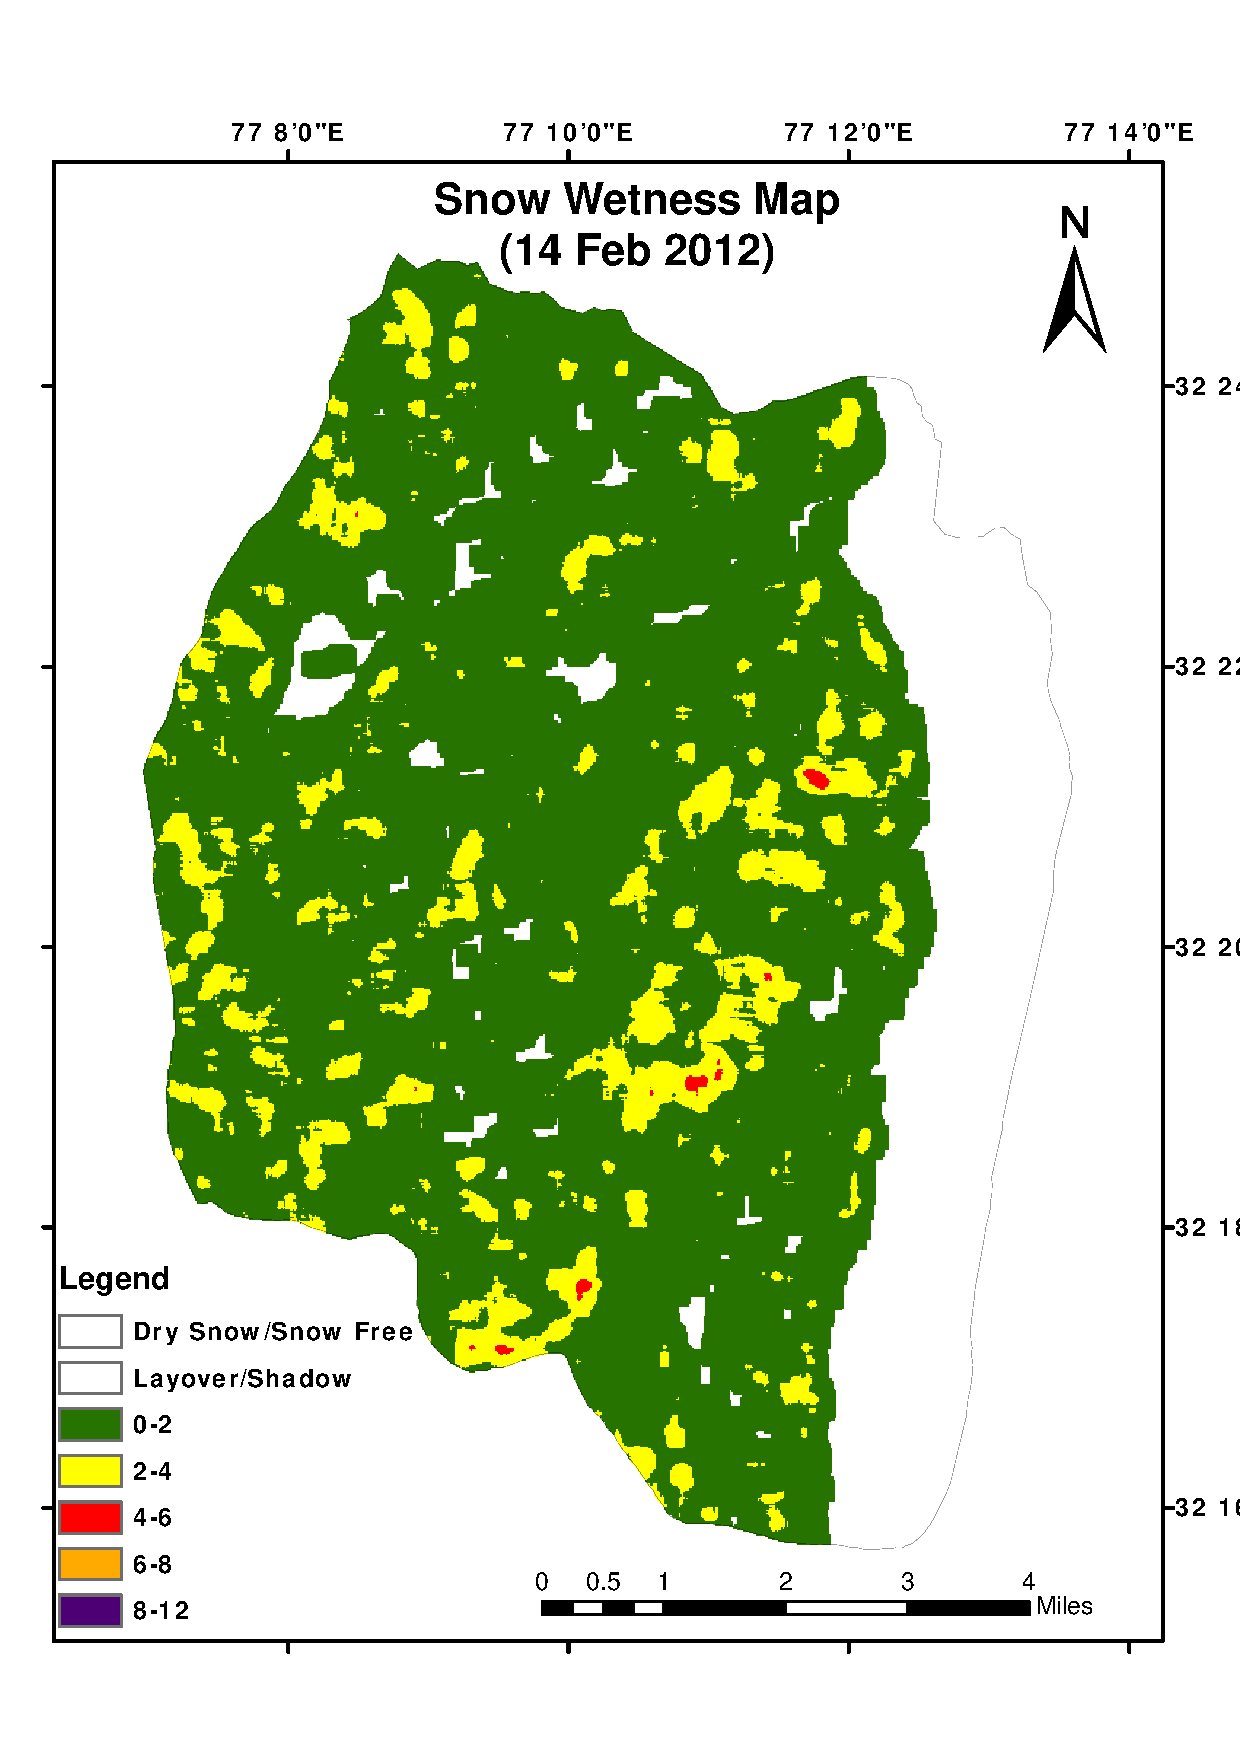
\includegraphics[width=0.49\textwidth]{Figures/14Feb2012}}
%	\subfloat[]{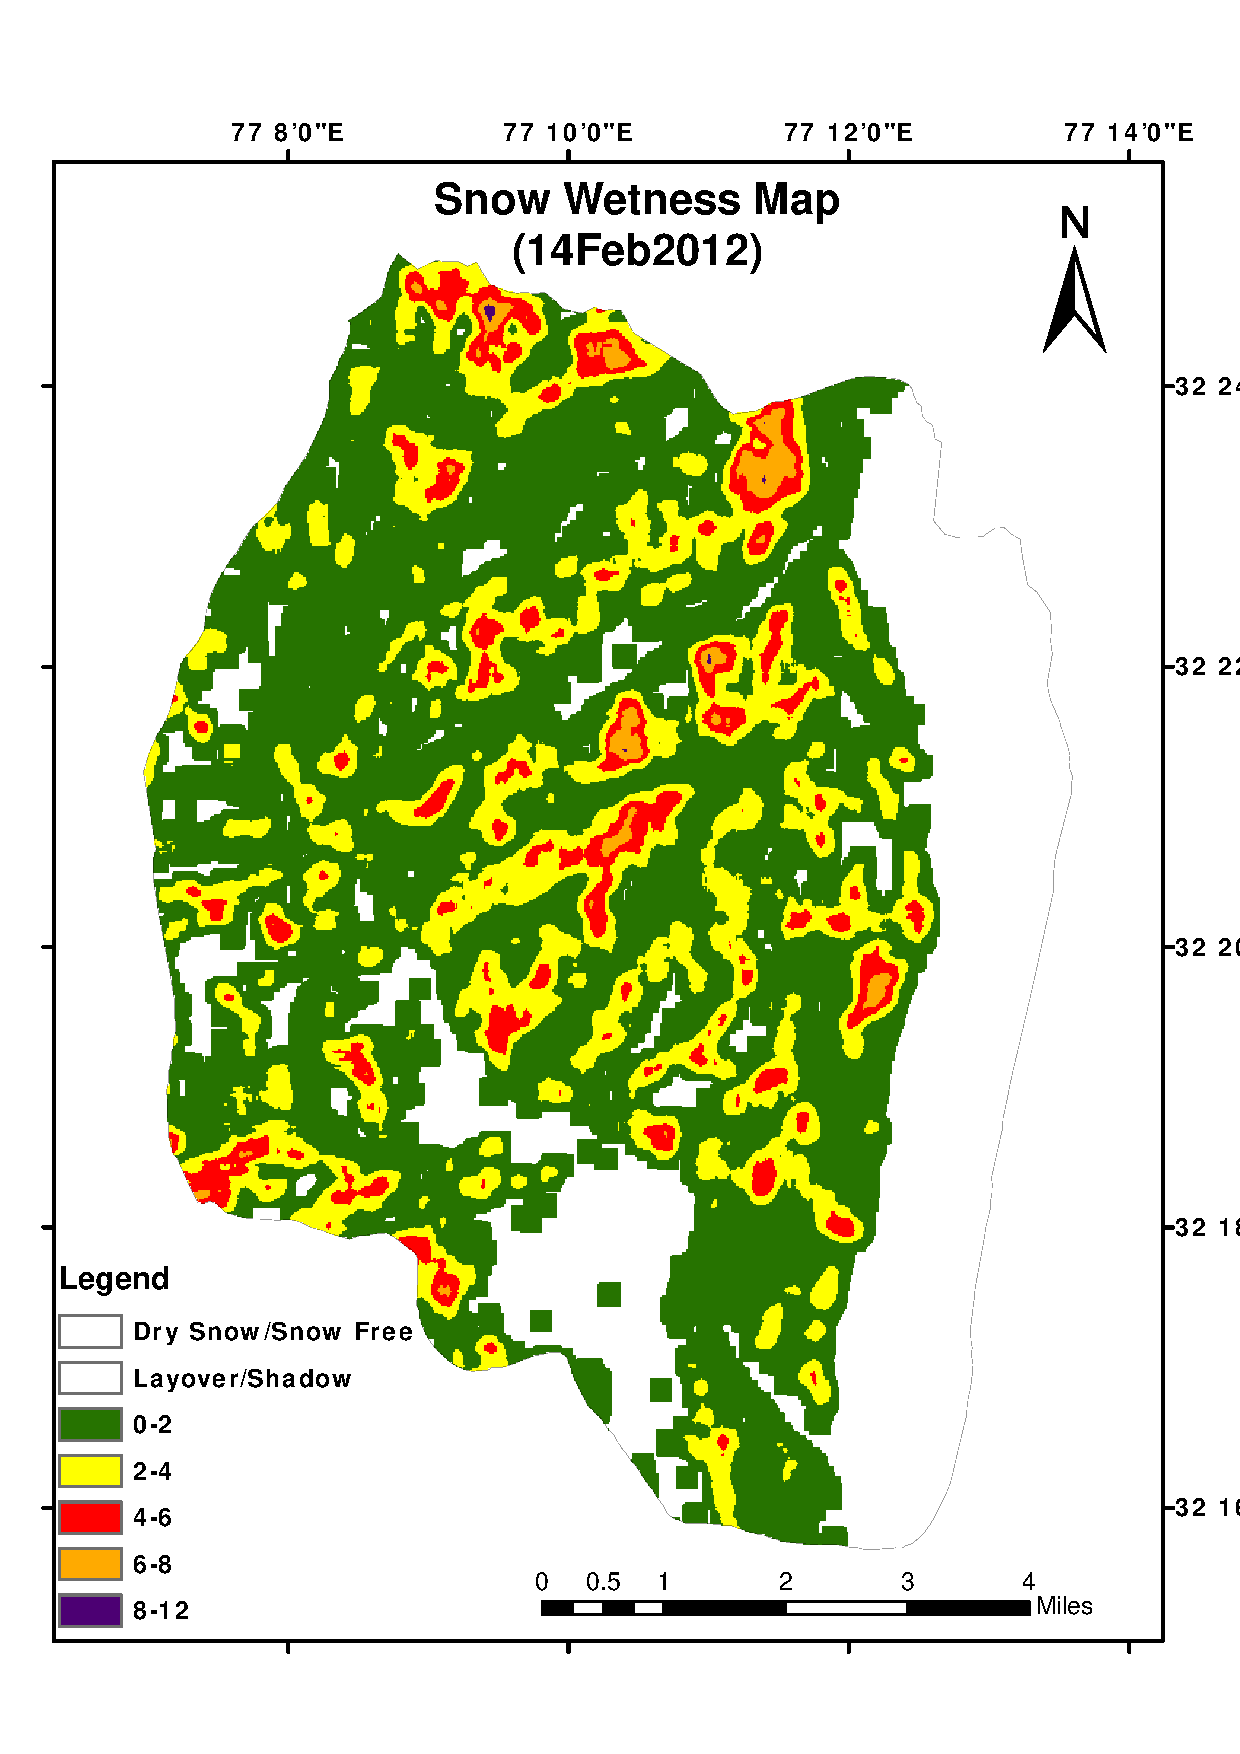
\includegraphics[width=0.49\textwidth]{Figures/14Feb2012_shi}}
%	\caption{Comparison of the snow wetness maps (in $\%$ volume) derived from (a) the proposed and (b) the Shi~-Dozier method. The white blank portion on the right hand side of the map is due to out of data coverage.}
%	\label{fig:proposed_shi_dozier_results}
%\end{figure*}
%
%\begin{figure*}[!th]
%	\centering
%	\subfloat[]{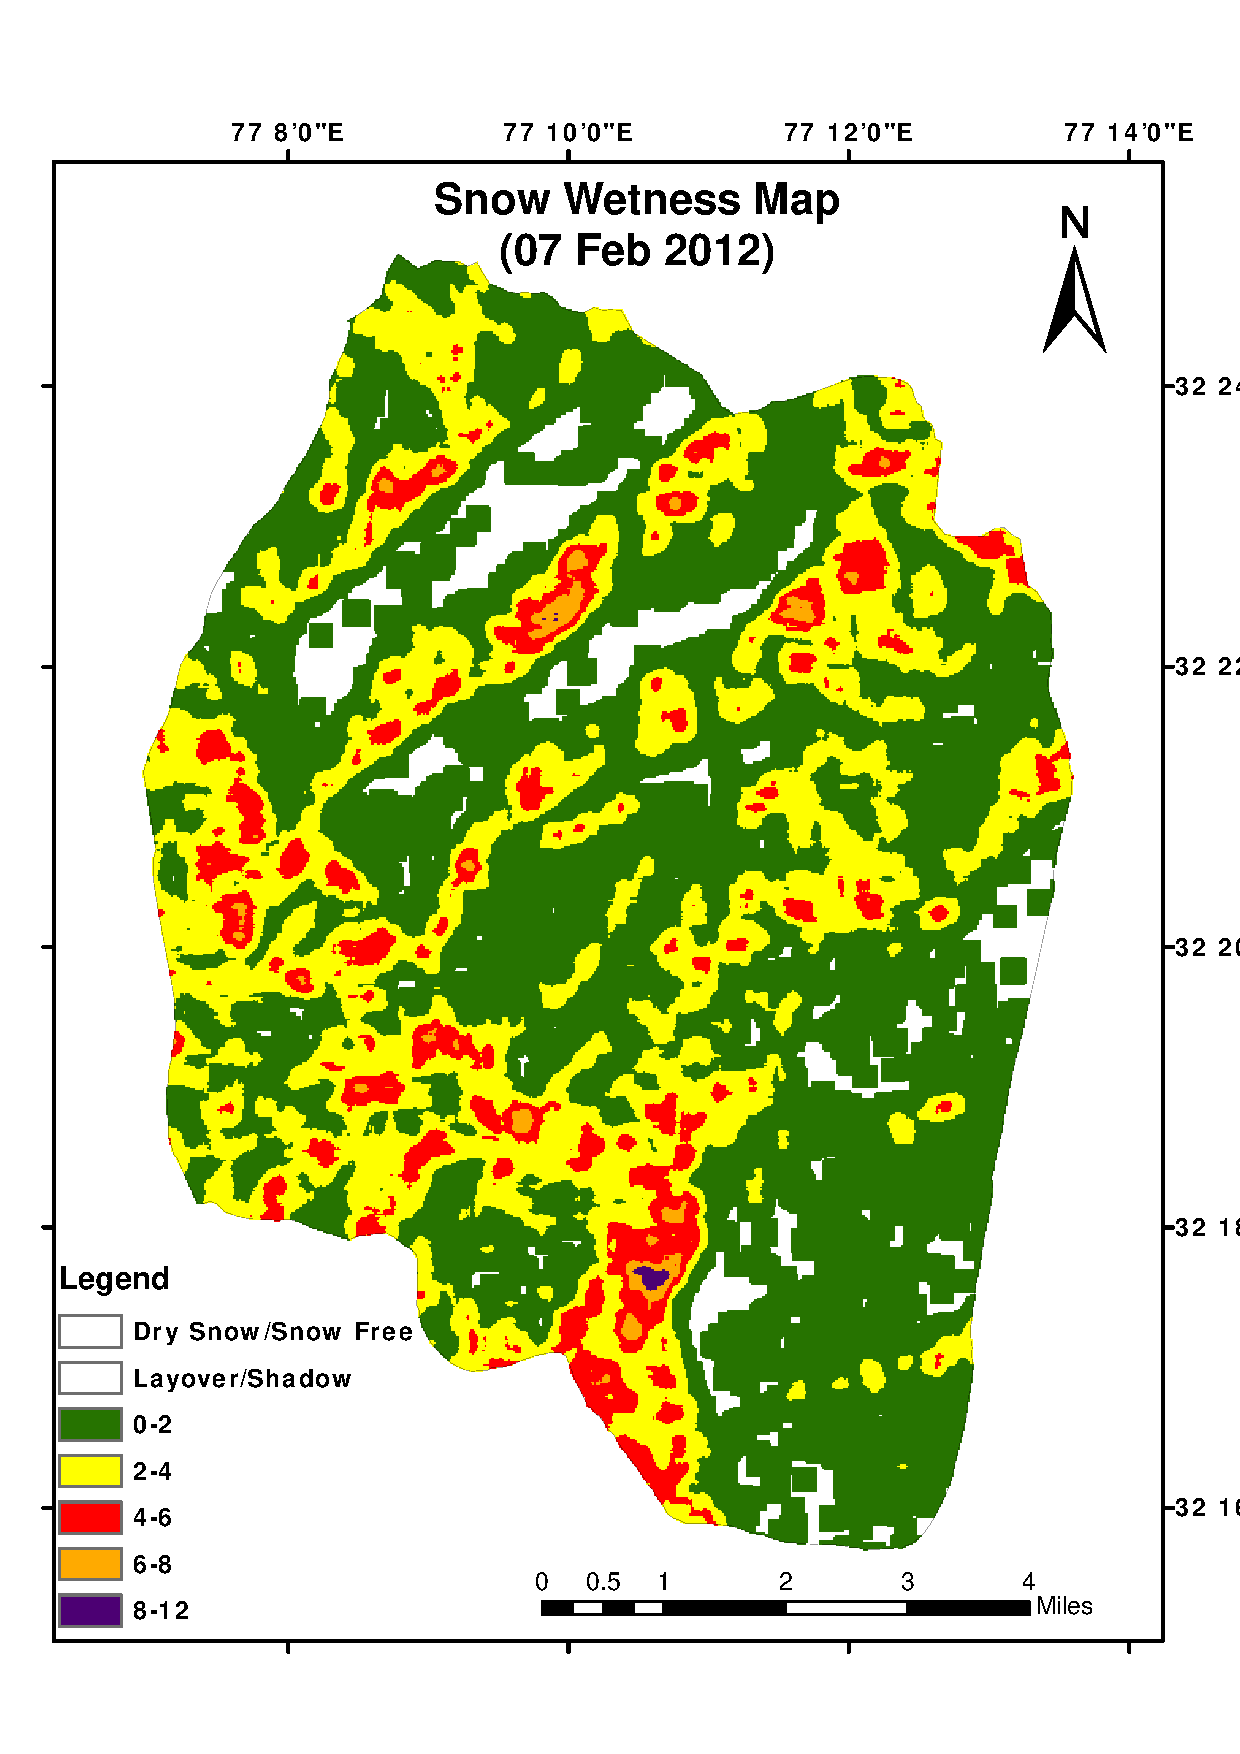
\includegraphics[width=0.5\textwidth]{Figures/07Feb2012}} 
%	\subfloat[]{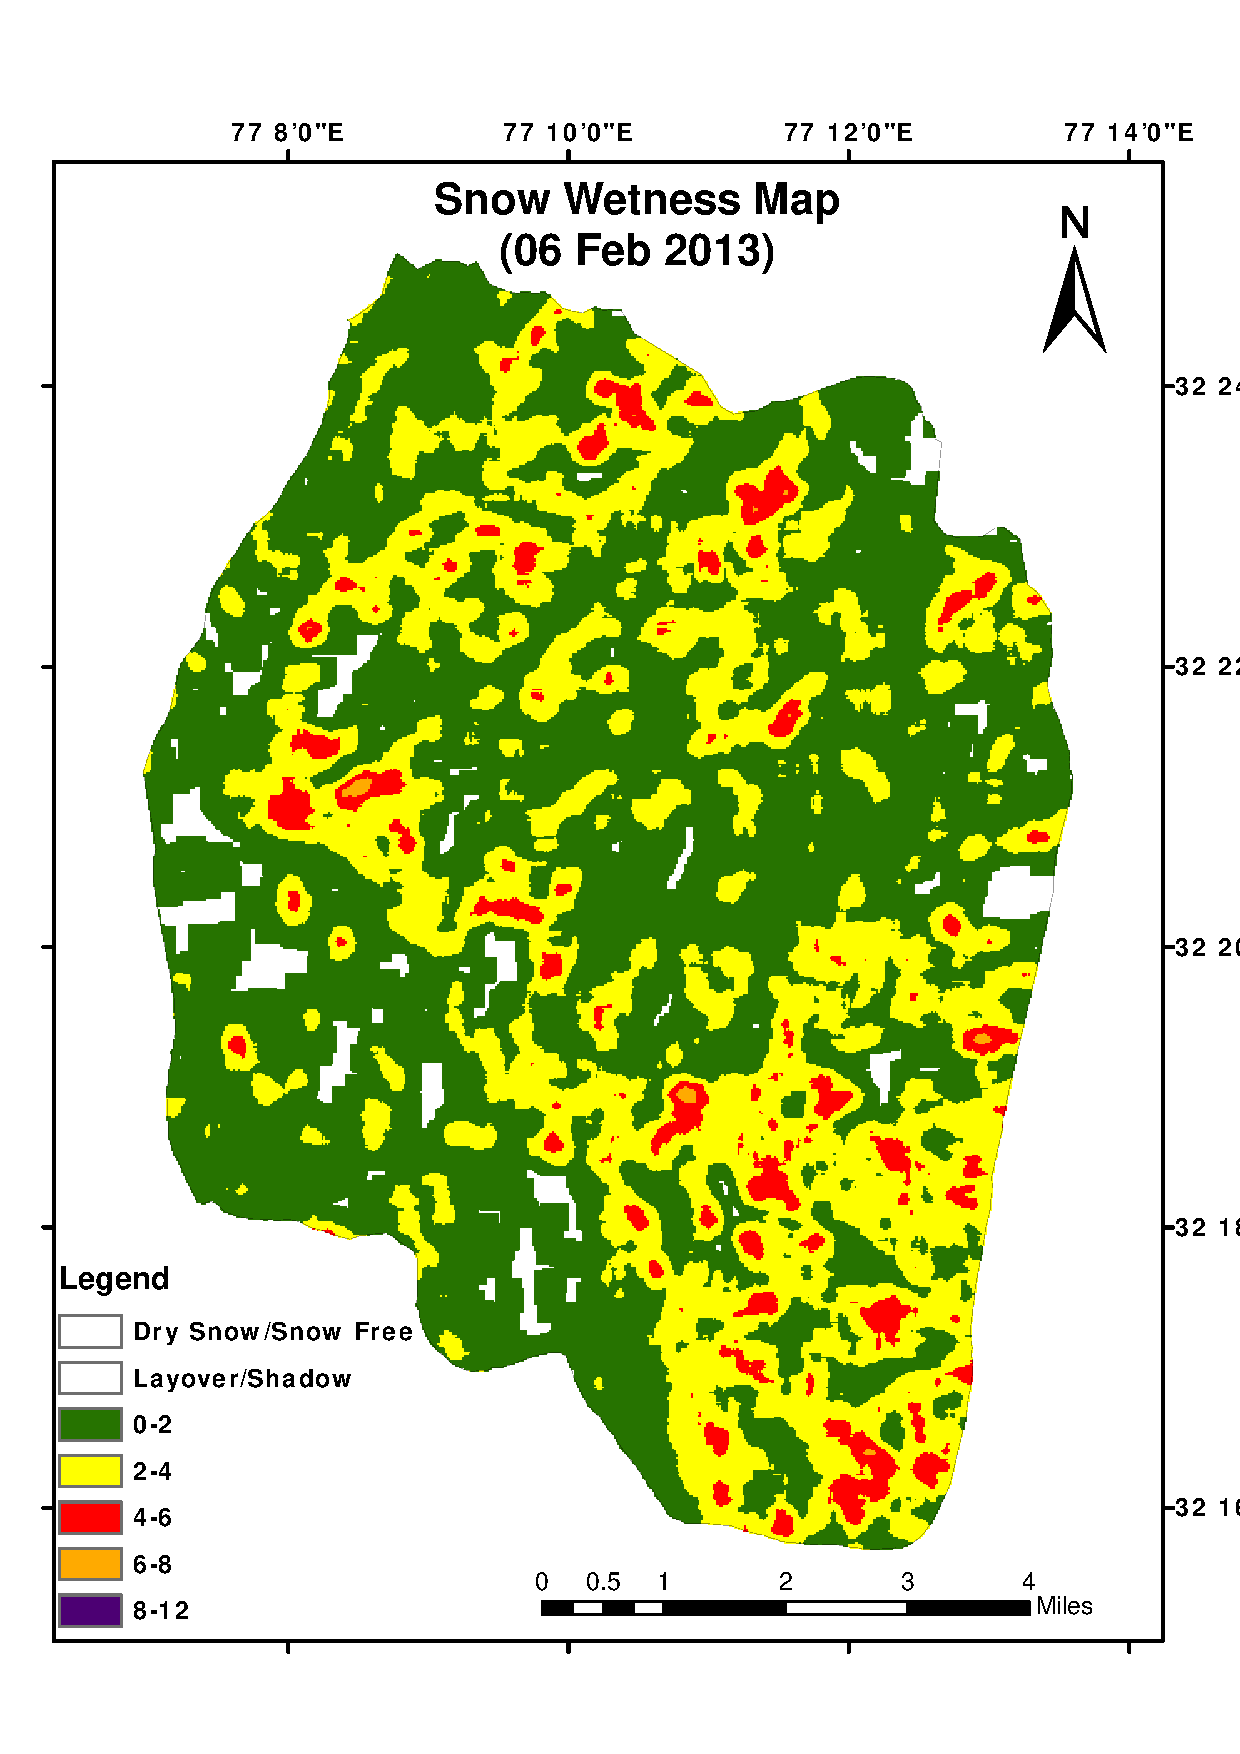
\includegraphics[width=0.5\textwidth]{Figures/06Feb2013}} 
%	\caption{Snow wetness maps (in $\%$ volume) derived from the proposed model.} 
%	\label{fig:proposed_results}
%\end{figure*}
%
%
%\begin{figure*}[!th]
%	\centering
%	\subfloat[]{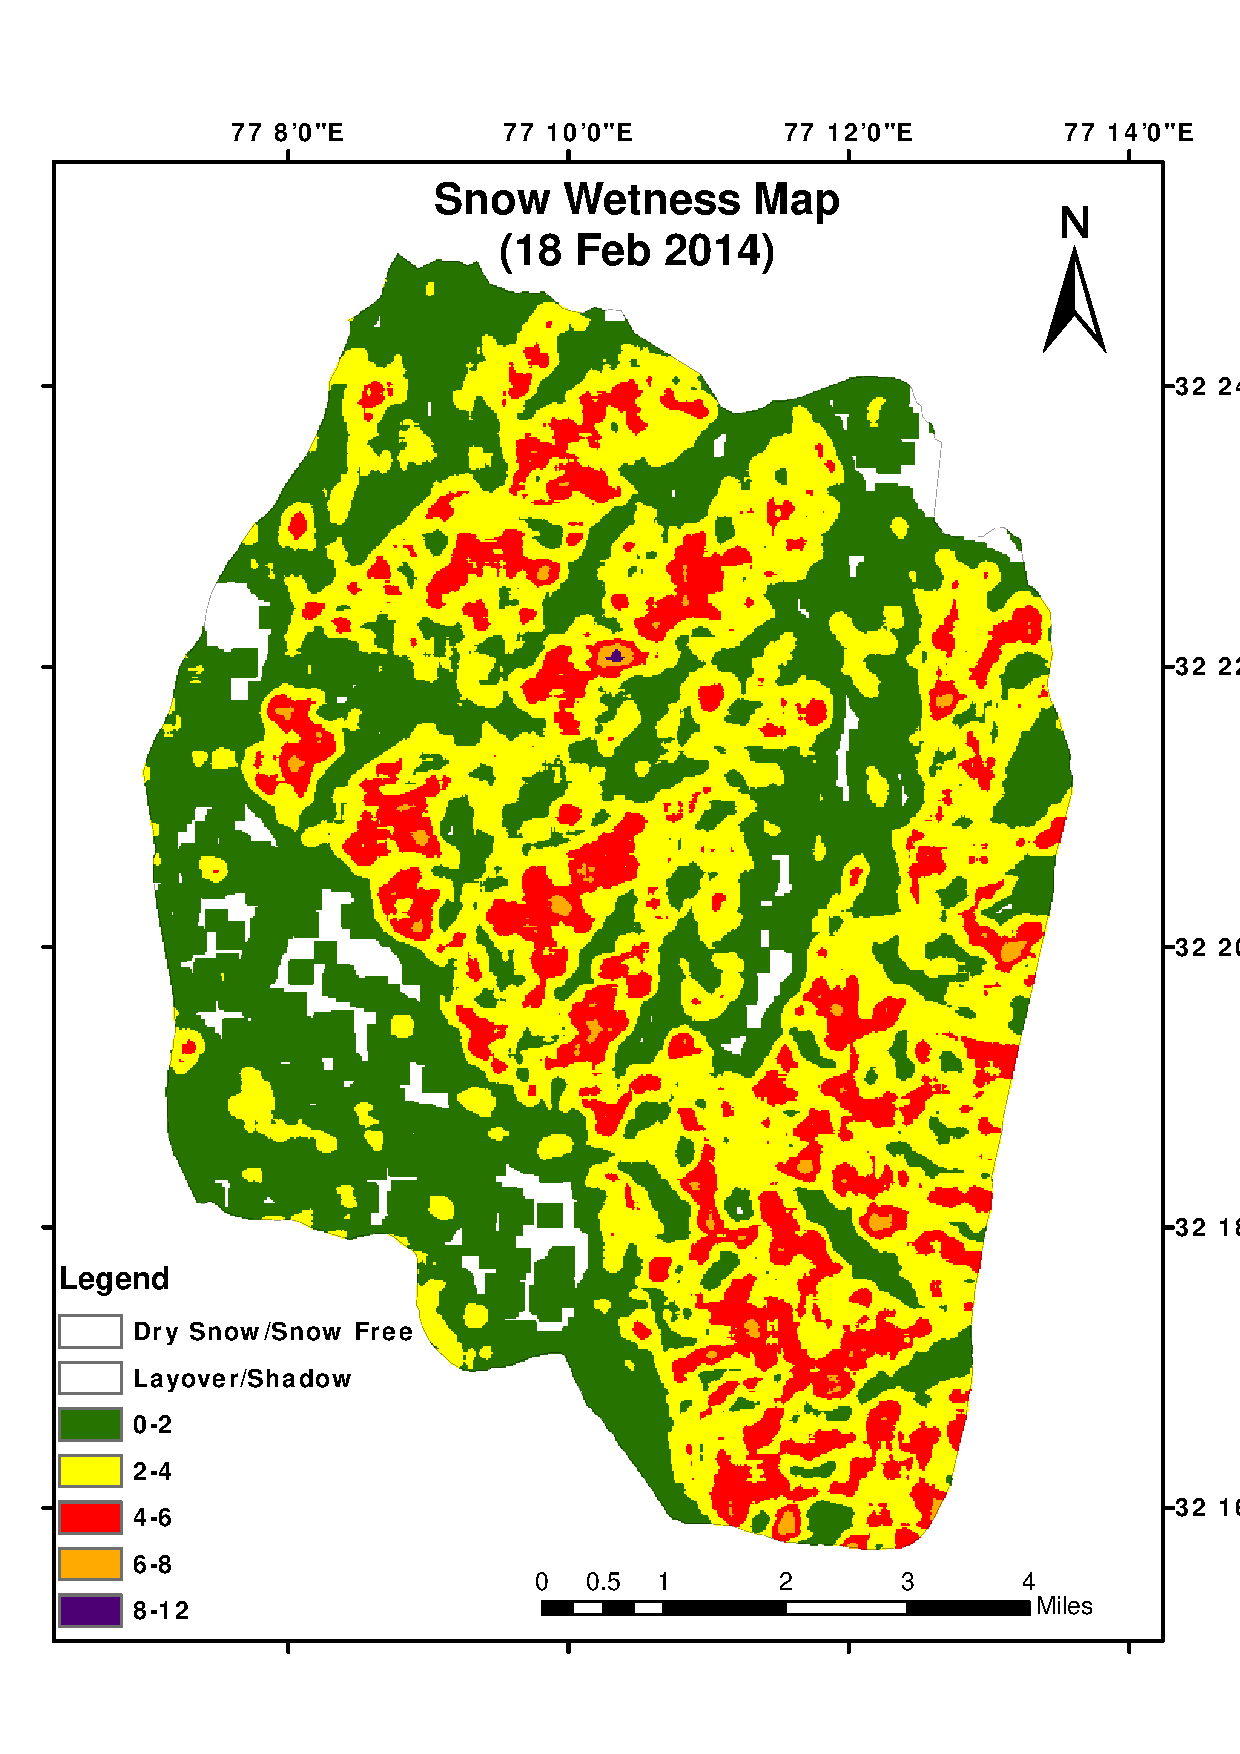
\includegraphics[width=0.5\textwidth]{Figures/18Feb2014}}
%	\subfloat[]{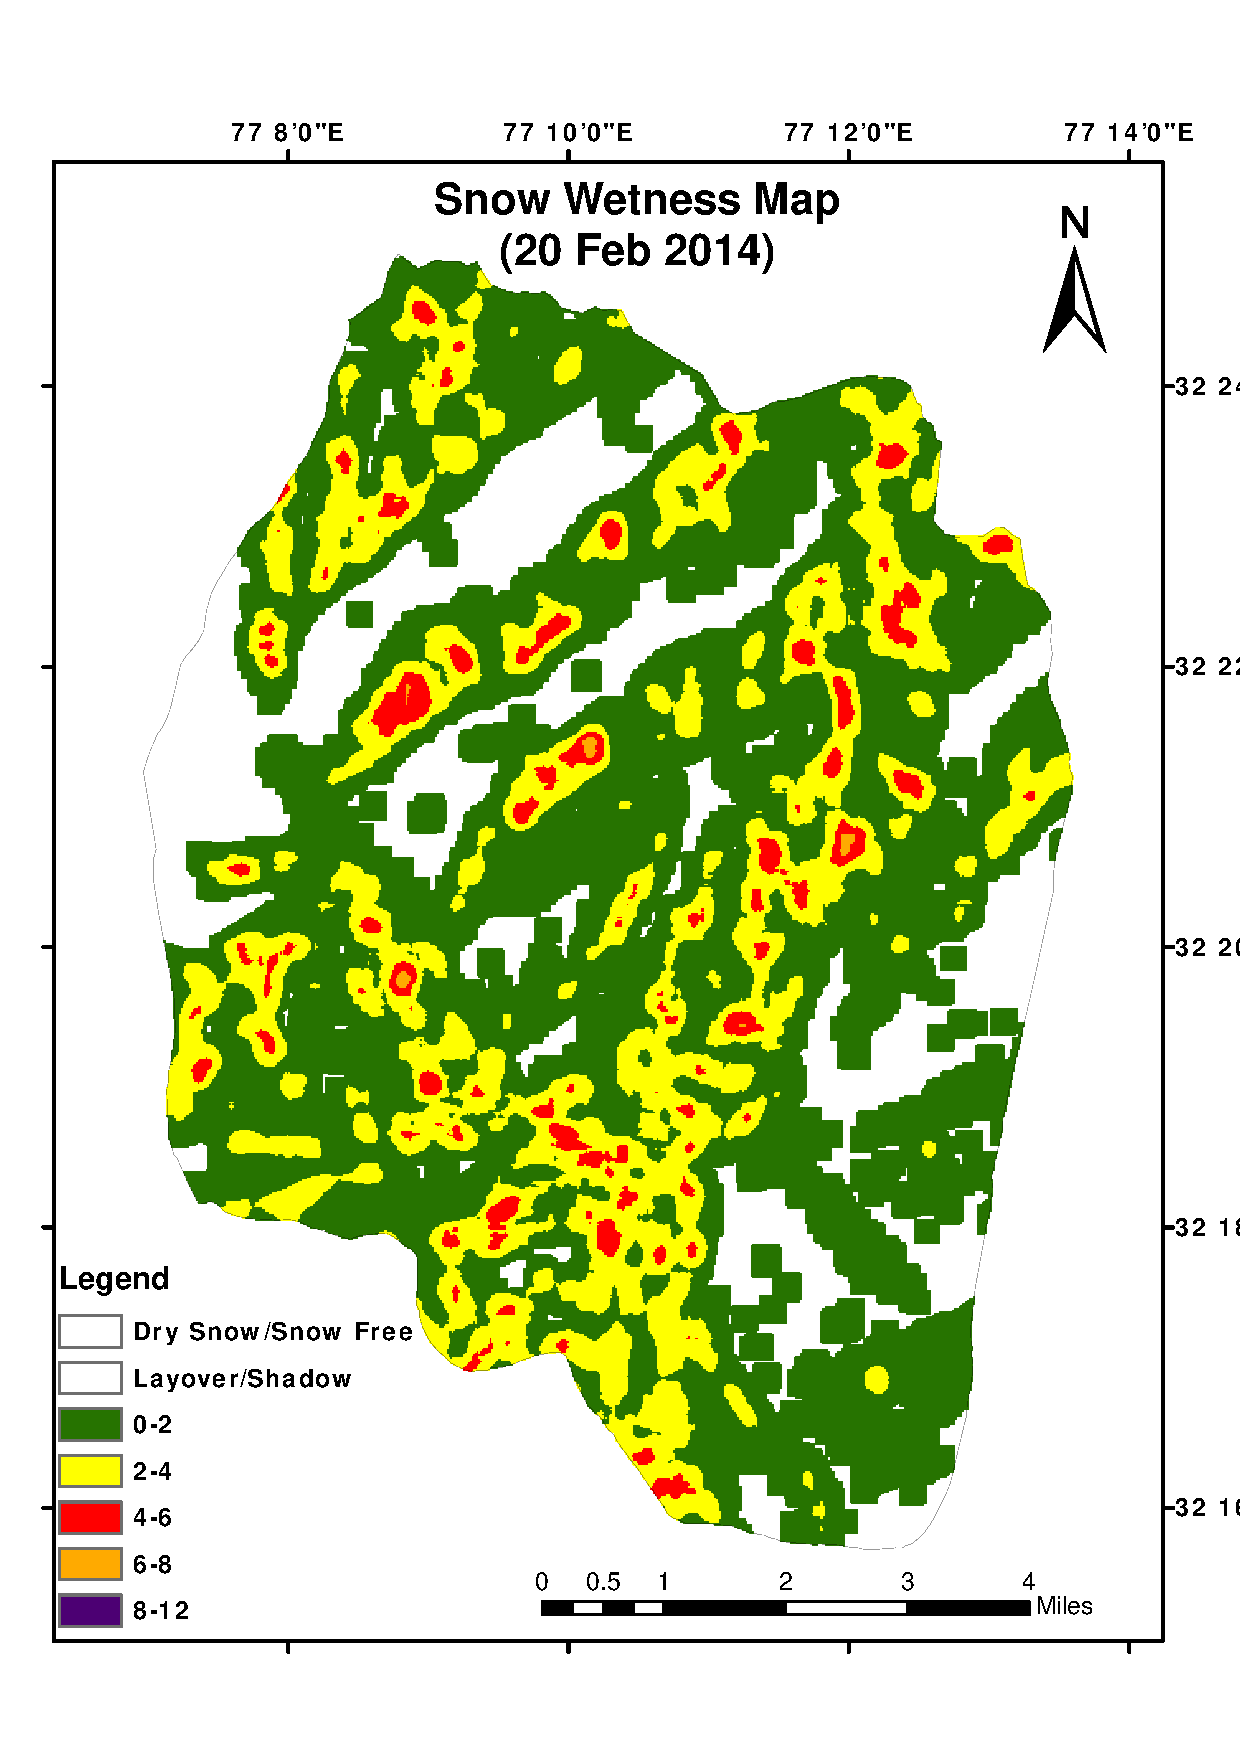
\includegraphics[width=0.5\textwidth]{Figures/20Feb2014}}
%	\caption{Snow wetness maps (in $\%$ volume) derived from the proposed model. RADARSAT-2 Data and Products ©MacDonald, Dettwiler and Associates Ltd. (2014) $–$ All Rights Reserved. RADARSAT is an official trademark of the Canadian Space Agency} 
%	\label{fig:proposed_results1}
%\end{figure*}
%
%%\begin{figure*}[!th]
%%\centering
%%\includegraphics[width=\textwidth]{validation_plot_1}
%%\caption{Comparison of the estimated snow wetness by the proposed and the Shi~-Dozier method with the in-situ measurements. Values indicated by Red *: proposed method and Blue +: Shi-Dozier.}
%%\label{fig:validation_plot}
%%\end{figure*}
%\begin{figure*}[!th]
%	\centering
%	\subfloat[]{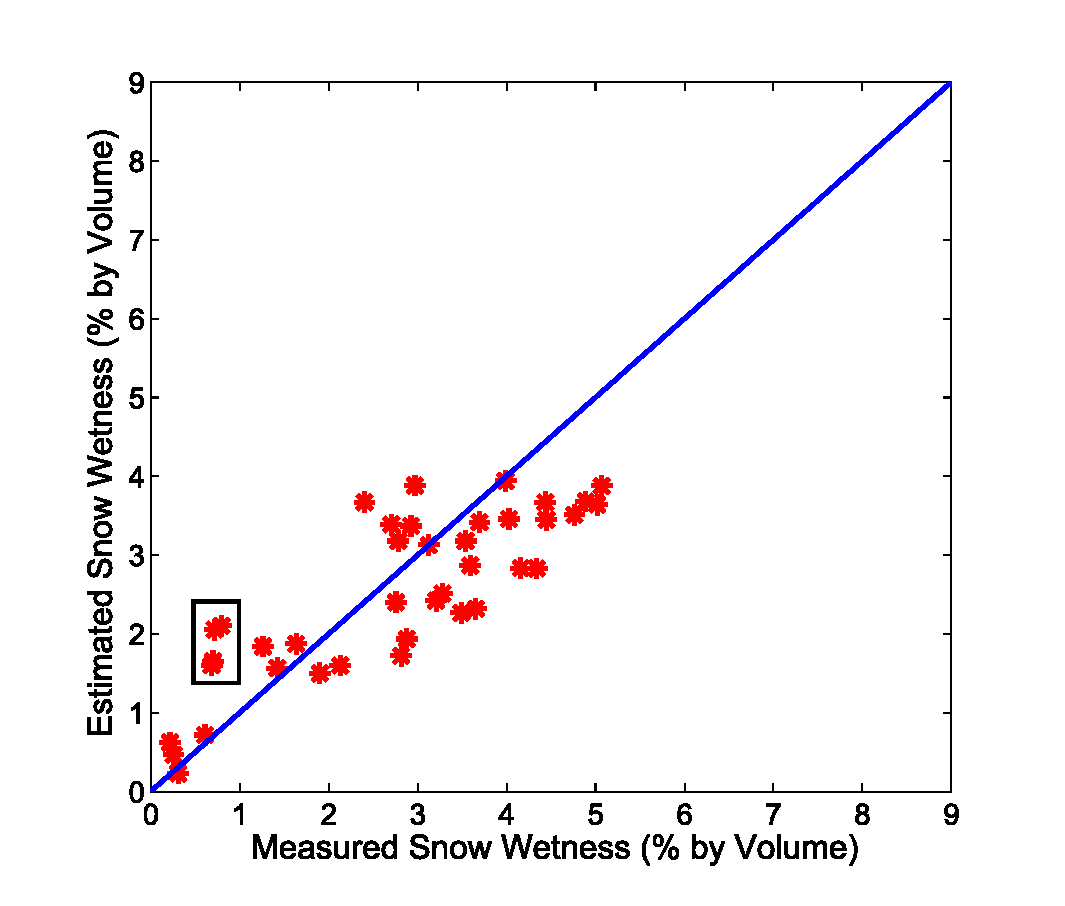
\includegraphics[width=0.5\textwidth]{Figures/validation_plot_proposed}}
%	\subfloat[]{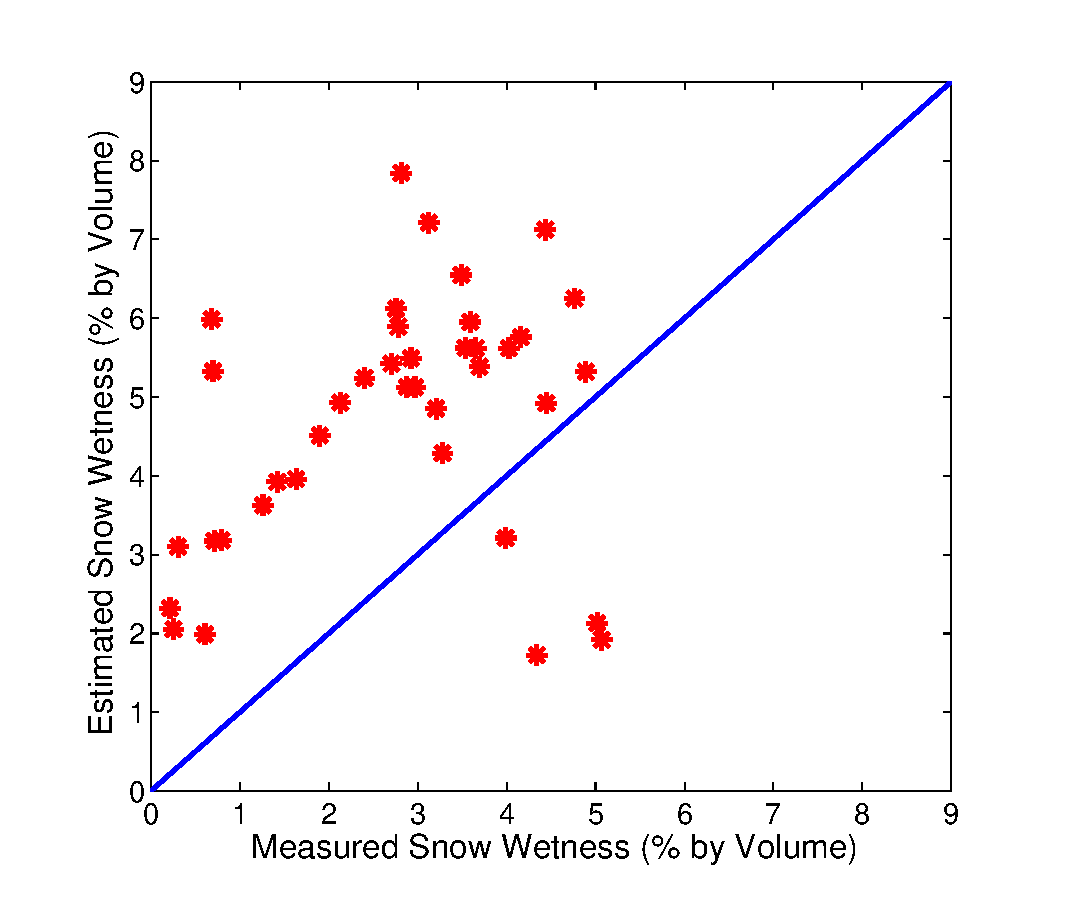
\includegraphics[width=0.5\textwidth]{Figures/validation_plot_shi}}
%	\caption{Comparison of the estimated snow wetness by (a) the newly proposed and (b) the existing Shi~-Dozier methods along with in-situ measurements.} 
%	\label{fig:validation_plot}
%\end{figure*}
%
%In the Indian Himalayan region the snowfall generally occurs during December to March from an altitude of 2000 m above the mean sea level. The mean minimum temperature in the month of January is around -15$^\circ$C-0$^\circ$C and the mean maximum temperature in the month of June is around 20$^\circ$C-30$^\circ$C. The expected snow wetness during Jan-Feb is around 2--6 $\%$ by volume because of fresh snowfall and average minimum temperature. 
%
%The surface and the volume snow wetness estimated by the proposed model for the 8 Feb 2013 data is shown in Fig.~\ref{fig:effective_snow_wetness}(a)-(b) respectively. The effective snow wetness map for 8 Feb 2013 data shown in Fig.~\ref{fig:effective_snow_wetness}(c) shows that most of the snow cover in the study area has a wetness in the range of 2--4$\%$ by volume. The minimum temperature recorded at the Bhang, Solang and Dhundi observatories were -~3$^\circ$C, -~7.5$^\circ$C and -~7$^\circ$C respectively. There was a 11 cm snow melt observed on the previous day (7 Feb 2013) due to a maximum temperature of 11$^\circ$C recorded at the Bhang observatory. However, the surface snow would have refrozen during the acquisition because of the recorded low temperature (-~3$^\circ$C). For cases with clear nights and temperatures close or below 0$^\circ$C, radiative emission from the snow surface (and also volume) causes a refreeze of the snow surface. The snow surface can freeze many centimeter deep during night, while the lower lying snow volume is still wet. Therefore, especially for acquisitions in the early morning hours, a higher contribution from the snow volume is expected. This is clearly observed from the estimation that the volume snow wetness is higher than the surface snow wetness. The scattering power plot~\ref{fig:effective_snow_wetness}(d), shows that the volume scattering power is higher than that of the surface. A similar trend in the estimated snow wetness and the observatory measurements is noticed on 20 Feb 2014 data (Fig.~\ref{fig:proposed_results1}(b)).
%
%The snow wetness map derived by the proposed model for the 14th Feb 2012 data over the study area (Fig.~\ref{fig:proposed_shi_dozier_results}(a)) shows low wetness values (0--2$\%$ by volume). The area was completely covered with dry snow and around 32 cm snowfall was recorded from 13th Feb evening to 14th Feb morning. The snow depth was around 300 cm over the Dhundi observatory and the temperature recorded was around -5$^\circ$C over the study area during the data acquisition. The estimated snow wetness results by the proposed model is in complete agreement with the in-situ measurements and is also in accordance to the field conditions. In comparison it can be seen that the estimated snow wetness map (Fig.~\ref{fig:proposed_shi_dozier_results}(b)) for the same data by the existing Shi-~Dozier method shows an over estimation of the wetness values compared to the in-situ measurements. 
%
%The snow wetness map for 7 Feb 2012 (Fig.~\ref{fig:proposed_results}(a)) data shows that the wetness is in the range of 2--3$\%$ around the Bhang observatory. During this descending pass acquisition, the in-situ measurements were collected around the Bhang observatory and the temperature was recorded around -~2$^\circ$C. The estimated wetness values have a decent concurrence with the field data collected in near-real time with the satellite pass. In the following year, the effective snow wetness was estimated for 6 and 8 Feb 2013 datasets. The snow wetness map derived from the proposed model for the 6 Feb data (Fig.~\ref{fig:proposed_results}(b)) shows that the wetness over the Bhang observatory region is around 3--6$\%$ with the maximum temperature of 4$^\circ$C. The wetness is around 1--3$\%$ over the Solang and the Dhundhi observatories where the maximum temperatures were recorded at 1.5$^\circ$C and 1$^\circ$C respectively along with a fresh snowfall on that day. 
%
%The effective snow wetness map for 18 Feb 2014 is shown in Fig.~\ref{fig:proposed_results1}(a) which is derived using the weighted average shows that the wetness is in the range of 3--6$\%$ over the study area. The maximum temperature for the day was recorded around 17$^\circ$C, 14$^\circ$C and 8$^\circ$C in the Bhang, Solang and Dhundi observatories respectively. Due to this high temperature there was a melting of 6 cm, 11 cm and 7 cm of snow within a span of less than 12 hours recorded at the three observatories respectively. This  can be clearly seen in the effective snow wetness map Fig.~\ref{fig:proposed_results1}(a) which is obtained from the surface (6--9$\%$) and the volume (3--8$\%$) snow wetness maps. This may be due to the melting of snow surface which subsequently percolates into the snowpack thereby increasing the volume wetness.
%
%A total of 40 in-situ measurements were collected in near-real time with the satellite data for three consecutive years to validate the proposed snow wetness estimation algorithm. The snow wetness estimated by the proposed and the Shi-Dozier algorithms along with in-situ measurements are plotted in Fig.~\ref{fig:validation_plot}(a) and (b) respectively. Particularly for low wetness condition ($<$ 3.5$\%$), the proposed model closely follows the in-situ measurements than the Shi-Dozier method. However, for most of the cases the Shi-Dozier method overestimate the snow wetness. The three in-situ measurements on 7 Feb 2012 over the Dhundi observatory were collected around six hours after the satellite pass. Due to this, the overestimation in the snow wetness is clearly seen in Fig.~\ref{fig:validation_plot}(a) marked within the black box.
%
%\section{Conclusion}
%In this chapter, a new model has been proposed to estimate snow wetness from full polarimetric SAR data.  The proposed model was applied to six Radarsat-2 fine resolution full-polarimetric data sets acquired over the Indian Himalayan region for three consecutive years. The results were comparable to the near real time in-situ measurements. The high accuracy of the proposed model is due to the utilization of the complete information from full polarimetric SAR data. The double unitary rotation of the full-polarimetric data has compensated the azimuth and the range slope effects which are predominant in mountainous regions. The effective wetness of the snowpack is estimated by using the normalized surface and the volume scattering powers derived from the G4U model based decomposition technique. This effective averaging of the surface and volume snow wetness using scattering powers is essential to account for different snow conditions. The comparison of the snow wetness derived from the proposed and the Shi-Dozier methods with the ground measurements indicated that the absolute error at 95$\%$ confidence interval were 1.3$\%$ and 2.6$\%$ by volume respectively. The proposed method shows a better estimation of the snow wetness compared to the Shi-Dozzier method. In the future, the proposed model will be further improved to consider snow wetness under vegetation cover. Furthermore, the model will be tested with multi-frequency SAR polarimetric data. 
%
